\documentclass[conference]{IEEEtran}
\IEEEoverridecommandlockouts
\usepackage{algorithmic}
\usepackage{amsmath,amssymb,amsfonts}
\usepackage{cite}
\usepackage{graphicx}
\usepackage{hyperref}
\usepackage{svg}
\usepackage{textcomp}
\usepackage{xcolor}
\def\BibTeX{{\rm B\kern-.05em{\sc i\kern-.025em b}\kern-.08em
T\kern-.1667em\lower.7ex\hbox{E}\kern-.125emX}}

\usepackage{epstopdf}
\pdfminorversion=7 % Because epstopdf outputs as version 1.7

\begin{document}
    \title{
        Fruit Flies:\\
        Developing Flying Orchard Robots
    }

    \author{
        \IEEEauthorblockN{Michael Hegerhorst}
        \IEEEauthorblockA{michael.hegerhorst@gmail.com}
        \and
        \IEEEauthorblockN{Keaton Anderson}
        \IEEEauthorblockA{keatona379@gmail.com}
        \and
        \IEEEauthorblockN{Caleb Syndergaard}
        \IEEEauthorblockA{caleb.syndergaard@gmail.com}
    }

    \maketitle
% \thispagestyle{plain} and \pagestyle{plain} allow page numbers
    \thispagestyle{plain}
    \pagestyle{plain}

    \begin{abstract}
    Farmers face numerous challenges when maintaining their crops, one of which is
    knowing when their crops are ripe.
    In particular, orchards can be difficult to manage and fruit can hide in branches.
    There is a need to develop a technique to assist farmers in maintaining their
    orchards.
    Modern technologies provide ways to develop models to detect the ripeness of
    crops, such as apples.
    We developed an intelligence hierarchy to use flying drones to assist in the
    maintenance of orchards by identifying ripe apples.
\end{abstract}


% TODO: Split up by section
% Intro
% Methodology
% Results
% Conclusions
% Etc.
    \section{Introduction}
%  Present topic and goal
Farmers require a lot of land in order to grow their crops, and navigating this land is time consuming and difficult.
In the U.S., apple orchards take up over 382 thousand acres of land\cite{USApple}, requiring over 100 thousand workers\cite{USApple}. 
Our project focuses on helping farmer's manage crops across their many acres of land by making use of a drone equipped with machine learning models to 
find apples within the orchard and predict their ripeness and health. By avoiding the need for manual inspection of apples over this large area 
we can lower the time demand for farmer's, and provide a more standardized method of determining crop health by removing the subjectivity of human decision making.
Although the original scale of the product involved analysis of entire orchards, in order to meet our time constraints, we focused on training a drone to recognize, follow, and determine the ripeness of an apple. We succeeded in training a drone to recognize and follow an apple through the use of a Haar-Cascade model in conjunction with an support vector machine (SVM) to determine the apple's ripeness. This paper functions as a proof of concept and a starting point for future research into detecting fruit in trees and generating predictive yields.
\\

%  Existing research
% FIXME: MDH: We don't necessarily need all these sections. Feel free to add or
%     remove as desired.
    \section{Background}
\subsection{UAV's in Agriculture}
Although the concept of including Unarmed Aerial Vehicles (UAVs) in agriculture is a rather new concept, there has been some preliminary work done by other researchers on the subject.
Predominately, research conducted in this field has been investigative, rather than relying on actual experimentation.
An example of this is provided in "The influence of drone monitoring on crop health and harvest size", a paper outlining possible uses of drones in the agricultural scene \cite{Reinecke2017}.
During the course of the research conducted by the authors of the aforementioned study, they conducted two interviews. 
The first interview was with UVIRCO, a company "who specialize[s] in cameras and often fit them on drones" and Aerobatics, which is a drone manufacturing company \cite{Reinecke2017}.
The researchers made several conclusions that helped to contribute to our interest in the project.
For examples, they concluded, "drones can be equipped with a multispectral camera that can detect the water content underground, which can allow a farmer to determine if a crop row is parched or overhydrated" \cite{Reinecke2017}.
In addition to this, their findings showed that "drones can create a digital map of a field, detect problems with crop health, find missing livestock, find leaks in irrigation systems, detect the size and spread of fires and potentially spray pesticides" \cite{Reinecke2017}.
In another study conducted in 2017, the concept of using drones to monitor soil moisture levels to determine plant health and other information like possible irrigation system leaks \cite{Hassan2017}. In this paper, the authors discuss the alternative approaches of using satellite imaging to solve analagous problems and determined that the use of drones was "a potential step forward for possible future use in precision agriculture and irrigation scheduling" \cite{Hassan2017}.
\\
Because many of the applications of drones in agriculture require special cameras, such as "multispectral and thermal cameras", we sought to make use of standard imaging systems in conjunction with machine learning in order to lower the expense barrier an orchardist would need to cross to get a useful product \cite{Reinecke2017}.
In order do do so, we s

    \section{Methodology}
%  Subsection for each segment of the project?
\subsection{Robot Design}\label{subsec:robot-design}
For this project, we elected to use a flying Tello drone.
We chose a flying drone primarily because it can easily bring its camera into detection range of apples in a tree, regardless of height.
A flying drone also has the advantage of not disturbing or caring about the terrain, which may be muddy or bumpy in some orchards.

However, flying drones suffer from a number of disadvantages.
The two primary difficulties are the lack of computational power and the lack of battery life.
A typical drone is unable to remain in the air long enough to both approach apples and determine their ripeness, and are  additionally too slow to use some of the heavier models in a reasonable time-frame.
As such, in order to overcome these challenges we developed an intelligence hierarchy to only perform calculations as required, and offloaded these calculations to an external ``controller'' computer.

The intelligence hierarchy is outlined in \autoref{fig:intelligence-hierarchy}.
The controller starts by detecting if an apple if is in view, then proceeds to calculate its position relative to the apple and approach it.
Finally, models are used to detect the ripeness of the apple, as well as if it is rotten.

The data flow for the hierarchy can be seen in \autoref{fig:fruit-fly-model-diagram}.
Each step occurs sequentially, and the next one only occu
This setup removes the burden from the drone, while also minimizing the calculations done by the controller.


\begin{figure}[!htb]
    \fontsize{7}{5}\selectfont
    \centering
    \includegraphics[scale=0.8]
    {./figures/intelligence-hierarchy}
    \caption{
        The intelligence hierarchy used by the drone.
        Each layer is designed to minimize the work done by the controller so it does not perform expensive calculations except when needed.
    }
    \label{fig:intelligence-hierarchy}
\end{figure}

\begin{figure}[!htb]
    \fontsize{7}{5}\selectfont
    \centering
    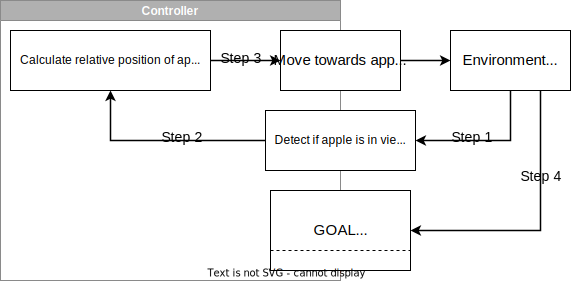
\includegraphics[width=\columnwidth,keepaspectratio]
    {./figures/fruit-fly-model-diagram}
    \caption{
        A data flow diagram of how the intelligence hierarchy works.
        The controller, which operates on another machine receives input from the drone's cameras and other sensors.
        This information is passed to a lightweight model, then to heavier models to operate the drone and determine fruit ripeness.
    }
    \label{fig:fruit-fly-model-diagram}
\end{figure}

\subsection{Initial Object \& Location Detection}\label{subsec:initial-object
-&-location-detection}
As the intelligence hierarchy demonstrates, the first component of our model needed
to be able to detect when an apple appeared in the drone's field of view.
We trained a lightweight convolutional neural network (CNN), that was based off of
MobileNet~\cite{Sandler2018,PyTorchMobileNet} in order to accomplish this.
In order to do this, we selected a Haar-Cascade model because of its lightweight
nature, simplicity, and its real-time object detection capabilities.\footnote{The
Haar-Cascade model was trained using a graphical user interface created by Amin
Ahmadi (\url{https://amin-ahmadi.com/cascade-trainer-gui/}).}
The data we used to train the model was a compilation of datasets such as the
Fruit360 dataset ~\cite{Fruit360}.
In addition to the positive images (images containing apples), a myriad of negative
images (images without apples) were used to train the model.
The negative images were selected based on specific characteristics we knew the model
would eventually encounter.
For example, we have a set of images that contain hands holding objects that aren't
apples, so that the model can differentiate between when someone
is holding an apple and when someone is holding a different object.
Another set of images that we included in the negative training data featured
different kinds of trees that didn't have apples in them.
These trees ranged from trees that were structurally similar to apple trees, but
didn't contain any apples, to trees that contained different kinds of fruit, like
oranges.
This was done with the express purpose of extensibility.
As the goal is to eventually introduce our model to an orchard, the drone will need
to be familiar with what a tree with or without apples looks like.
This helps ensure that the model will be effective when it enters into a production
environment.

\subsection{Ripeness Detection}
\subsubsection{Data}
The data for this model was a subset of the Fruits360 data set~\cite{Fruit360}.
Unable to find any suitable data sets showing a single apple species at different stages of ripeness, we settled for using two ripe, similar looking apple species.
In the Fruits360 data set~\cite{Fruit360}, we used crimson snow apples to represent ripe apples, and the data set's ``red 2'' apples to represent unripe apples. We  chose to use these since the two types had a very similar shape in their images, making the biggest variation between them the color which is what our model focuses on.

\subsubsection{Model}
The ripeness of an apple is determined by an SVM classifier model based on the HSV values of the apple image because it has been shown to be capable of having a high accuracy at fruit ripeness detection~\cite{HSVRipeness}.
The model takes an input feature vector based on the histogram calculation of an HSV image measuring $(100$pixels$\times100$pixels), Using OpenCV and python.
Within OpenCV, hue is a number from 0 to 179, inclusive, and saturation and value are both numbers from 0 to 255, inclusive.
These calculation values then get flattened down into a 1-dimensional feature vector storing 689 numbers. 
This feature vector is used as input for our SVM classifier. Below is an example of a ripe apple, and its HSV histogram calculation values. The $y$ value of each point of each line is the amount of times that value of H, S, or V appears in the image.\\
\begin{figure}[!htb]
    \fontsize{7}{5}\selectfont
    \centering
    \includegraphics[scale=0.7]
    {figures/Ripe Apple Example.jpg}
    \includegraphics[scale=.5]
    {figures/ripeness_features.png}
    \label{Ripe Apple Example}
    \caption{
        A ripe apple, and its associated HSV histogram calculations from the image preprocessing.
    }
\end{figure}

\subsubsection{Improvements}
Because we were unable to find data focused more specifically on detecting ripeness, 
one good way to improve the performance of our project would be to gather picture of both ripe and unripe variants of whatever apple species the drone would be targeting. 
To make this model production ready, it would likely require a new ripeness model to be trained for each species of apple targeted.
The model curre



    \section{Results}\label{sec:results}

\subsection{Model Performance}\label{subsec:model-performance}
Overall, the models developed as part of the intelligence hierarchy performed fairly
well.
\autoref{fig:apple-tree-mode-training-curve} demonstrates a learning curve for one of
the first-layer apple-in-view models.
The model was able to learn in fairly few epochs, and seemed to achieve fairly low loss.
A confusion matrix was then generate on a test set, the results of which can be seen
in \autoref{fig:apple-in-view-confusion-matrix}.

\begin{figure}[!htb]
    \centering
    \includegraphics[width=\columnwidth,keepaspectratio]
    {./figures/mobile_model_apple_trees_16its_2022-11-15_training_curve}
    \caption{
        Learning curve for a apple-in-view CNN.
        The model is a retrained version of MobileNet~\cite{Sandler2018,
            PyTorchMobileNet}, which is a more light-weight while still very powerful
        CNN.
        Loss is in mean squared error.
    }
    \label{fig:apple-tree-mode-training-curve}
\end{figure}

\begin{figure}[htb]
    \centering
    \includegraphics[width=\columnwidth,keepaspectratio]
    {./figures/confusion_matrix_All_Files_on_Dataset}
    \caption{
        The confusion matrix of the primary apple-in-view detection model on a test set.
        The column is the predicted label, while the row is the true label.
        A perfect model will have 0s in the top-right and bottom-left corner.
    }
    \label{fig:apple-in-view-confusion-matrix}
\end{figure}

While these initial models appear to perform well, as second round of tests from a
small, separate dataset consisting of hands holding apples was conducted and yielded
considerably worse results (see \autoref{fig:apple-in-hand-confusion-matrix}).
This is not only true for the apple-in-view layer models, but models at all levels of
the intelligence hierarchy.
We believe this is because the datasets used to train the models~\cite{Fruit360,
    Sultana2022} may not have been sufficiently diverse.
We attempted to enhance the dataset through curating web-scraped images, but the
models ultimately yielded the same results.
Given more time, we feel better data could be accumulated and better models developed.

\begin{figure}[htb]
    \centering
    \includegraphics[width=\columnwidth,keepaspectratio]
    {./figures/confusion_matrix_All_Files_on_Hands_with_Apples}
    \caption{
        The confusion matrix of the primary apple-in-view detection model on a new,
        apples-in-hand dataset.
        The column is the predicted label, while the row is the true label.
        A perfect model will have 0s in the top-right and bottom-left corner.
        Notice how the model fails to correctly classify the majority of images.
    }
    \label{fig:apple-in-hand-confusion-matrix}
\end{figure}

The ripeness prediction model had great performance, it was able to achieve a
validation and testing accuracy of $100\%$.
This could be because of our dataset.
We used 1272 images of two different apple species that were all taken in a very
controlled environment with small amounts of variance between each image.
A model similar to this one being used in a real world situation would likely perform
far worse.
A confusion matrix for this model is found in \autoref{fig:ripeness-confusion-matrix}.

\begin{figure}[htb]
    \centering
    \includegraphics[width=\columnwidth,keepaspectratio]
    {./figures/ripeness_confusion}
    \caption{
        The confusion matrix of the ripeness detection model when tested with unseen
        samples.
        The column is the predicted label, while the row is the true label.
    }
    \label{fig:ripeness-confusion-matrix}
\end{figure}

\subsection{Robot Performance}\label{subsec:robot-performance}
Even with their shortcomings, the models developed were sufficient for use with the
drone.
\autoref{fig:drone-haar-cascade} shows an image captured from the drone during its
movement phase.
The drone was able to detect and approach apples, as well as detect if they were ripe
and if they were rotten.

\begin{figure}[htb]
    \centering
    \includegraphics[scale=0.4,keepaspectratio]
    {./figures/haar-cascade-detection}
    \caption{
        An image taken through the drone camera during the
        calculate-relative-position phase of the intelligence hierarchy.
        A Haar-Cascade model is used to identify the apple's location and distance
        relative to the drone, after which the drone is able to approach the apple.
    }
    \label{fig:drone-haar-cascade}
\end{figure}

A drone-view demo of the robot can be found at \mbox{\url{https://youtu
.be/sJOU8Dehln0}}, as well as an alternative view at \mbox{\url{https://youtu
.be/6oxaGR8jjL8}}.
Additionally, a stitched video with both videos somewhat synced can be found at
\mbox{\url{https://youtu.be/YzhpWDfQMg0}}, and a playlist at \url{https://youtube
.com/playlist?list=PL0leTwxvw46LurvJJF6e5QOCOxjKpmtiN}.


    \section{Conclusions}
To reiterate what was shown throughout our paper, the goal of our research was to create a drone capable of multi-apple detection and enumeration.
Although we weren't able to create a product capable of accomplishing the initial goal, we were able to provide a ``proof of concept'' so to speak.
The models that we used were consistently lightweight and reportedly capable of performing with minimal training data. 
Although we experienced a decent amount of success using these models, we lacked the data, training time, and compute capacity to create a model that was consistently performant and accurate.
We suspect that given a larger, more diverse dataset, we would be able to produce more accurate models. 
We concluded that despite the shortcomings of a drone, such as short battery life
The code for the project can be found in~\cite{FruitFly}.



    \bibliographystyle{IEEEtran}
    \begin{small}
        \bibliography{references}
    \end{small}

\end{document}
